\documentclass[a4paper, 12pt]{article}

\usepackage{fontspec}
\usepackage{polyglossia}
\defaultfontfeatures{Ligatures=TeX}
\setdefaultlanguage{russian}
\setotherlanguage{english}
\setmainfont{Times New Roman}
\newfontfamily{\latinfont}{Times New Roman}
\newfontfamily{\cyrillicfont}{Times New Roman}
\newfontfamily{\cyrillicfonttt}{Courier New}

\usepackage{geometry}
\usepackage{amsmath}
\usepackage{amssymb}
\usepackage{amsfonts}
\usepackage{graphicx}
\usepackage{float}
\usepackage{wrapfig}
\usepackage{subcaption}
%\usepackage[caption=false]{subfig}
\geometry{right=20mm}
\geometry{left=20mm}
\geometry{top=20mm}
\geometry{bottom=20mm}

\usepackage{indentfirst}
\usepackage[outputdir=auxiliary]{minted}

\graphicspath{{../img/}}
\DeclareMathOperator{\R}{\mathbb{R}}
\DeclareMathOperator{\C}{\mathbb{C}}
\renewcommand{\Re}{\mathrm{Re}}
\renewcommand{\Im}{\mathrm{Im}}


\begin{document}
    \begin{titlepage}
    \begin{center}
        \textit{МИНИСТЕРСТВО ОБРАЗОВАНИЯ И НАУКИ\\
        РОССИЙСКОЙ ФЕДЕРАЦИИ}
        \vspace{1ex}

        федеральное государственное бюджетное образовательное учреждение\\
        высшего профессионального образования
        \vspace{1ex}

        \textbf{САНКТ-ПЕТЕРБУРГСКИЙ НАЦИОНАЛЬНЫЙ ИССЛЕДОВАТЕЛЬСКИЙ УНИВЕРСИТЕТ ИТМО}
        \vspace{13ex}

        Лабораторная работа №3\\
        <<Динамика нелинейных систем>>\\
        по дисциплине <<Моделирование технических систем>>\\
        \vspace{1em}
        Вариант 3\\
    \end{center}
    \vspace{14em}
    \begin{flushright}
        \noindent
        Выполнили:\\
        студенты гр. R4133c\\
        Борисов М. В.\\
        Симонов П.\\
        Мацуганов А. И.\\
        \vspace{1em}
        Преподаватель:\\
        Семенов Д. М.
    \end{flushright}
    \vfill
    \begin{center}
        \large{Санкт-Петербург}\\
        2021 г.\\
    \end{center}
\end{titlepage}

    \setcounter{page}{2}
    \setlength{\parindent}{0pt}

    \section*{Задание 1}
    Дана каноническая модель системы в пространстве состояний.
    \begin{equation*}
        \left\{
        \begin{aligned}
            \dot{x} =& Ax + bu\\
            y =& Cx
        \end{aligned}
        \right.
    \end{equation*}
    Перейти к функциональной модели "вход-выход" и построить передаточную функцию системы.

    \subsection*{Дано}
    \begin{equation*}
        A =
        \begin{bmatrix}
            1& 2& 3 \\
            0& 1& -1\\
            1& 0& -1
        \end{bmatrix}
        , b =
        \begin{bmatrix}
            0\\
            0\\
            1
        \end{bmatrix}
        , C =
        \begin{bmatrix}
            0& 0& 1
        \end{bmatrix}
        .
    \end{equation*}

    \subsection*{Решение}
    Передаточная функция системы выражается известным соотношением
    \begin{equation}
        \label{eq:Ws}
        W(s) = C(sI - A)^{-1}b
    \end{equation}

    Подставляя в \ref{eq:Ws} данные задания получаем

    \begin{equation*}
        W(s) =
        \begin{bmatrix}
            0& 0& 1
        \end{bmatrix}
        \left(
        s
        \begin{bmatrix}
            1& 0& 0\\
            0& 1& 0\\
            0& 0& 1
        \end{bmatrix}
        -
        \begin{bmatrix}
            1& 2& 3 \\
            0& 1& -1\\
            1& 0& -1
        \end{bmatrix}
        \right)^{-1}
        \begin{bmatrix}
            0\\
            0\\
            1
        \end{bmatrix}
        =\dfrac{s^2 -2s + 1}{s^3 + s^2 +4s -6}
    \end{equation*}

    Из полученного выражения легко получить систему по модели "вход-выход", зная что
    \begin{equation*}
        \begin{aligned}
            a(s)y &= b(s)u\\
            W(s) &= \dfrac{b(s)}{a(s)}
        \end{aligned}
    \end{equation*}

    Получаем
    \begin{equation*}
        \dddot{y} + \ddot{y} + 4\dot{y} - 6y = \ddot{u}-2\dot{u} +u
    \end{equation*}

    \section*{Задание 2}
    Дана функциональная модель системы в пространстве "вход-выход" с нулевыми начальными данными.
    Перейти к канонической модели в пространстве состояний.

    \subsection*{Дано}
    \begin{equation*}
        \dddot{y} - 4\ddot{y} + 3\dot{y} - 4y = \ddot{u} - 2\dot{u} + u
    \end{equation*}

    \subsection*{Решение}
    Систему вида \[\dddot{y} + a_{1}\ddot{y} + a_{2}\dot{y} + a_{3}y = b_{1}\ddot{u} + b_{2}\dot{u} + b_{3}u\]
    легко представить её в виде модели в пространстве состояний составив соответствующие матрицы $A$, $B$ и $C$
    следующим образом:

    \begin{equation*}
        A =
        \begin{bmatrix}
            -a_1& 1& 0\\
            -a_2& 0& 1\\
            -a_3& 0& 0
        \end{bmatrix}
        , B =
        \begin{bmatrix}
            b_1\\
            b_2\\
            b_3
        \end{bmatrix}
        , C =
        \begin{bmatrix}
            1& 0& 0
        \end{bmatrix}
    \end{equation*}

    Подставляя это в систему
    \begin{equation*}
        \left\{
        \begin{aligned}
            \dot{x} &= Ax + bu\\
            y &= Cx
        \end{aligned}
        \right.
    \end{equation*}
    получим
    \begin{equation*}
        \left\{
        \begin{aligned}
            \dot{x_{1}} &= 4x_{1} + x_{2} + u\\
            \dot{x_{2}} &= -3x_{1} + x_{3} - 2u\\
            \dot{x_{3}} &= 4x_{1} + u\\
            y &= x_1
        \end{aligned}
        \right.
    \end{equation*}

    \section*{Задание 3}
    Дана система в пространстве состояний \[\dot{x} = Ax + Bu\], где $x \in \mathbb{R}^3$, $B$ -- единичная матрица
    размера $3 \times 3$.

    \begin{enumerate}
        \item Промоделировать данную систему в MATLAB. Вывести графики для каждой переменной от времени.
        \item Найти собственные числа матрицы $A$, убедиться в неустойчивости системы
        \item Найти границу коэффициента усиления $k^*$ такую, что при любых $k < k^*$ регулятор вида $u = kx$ будет
        обеспечивать устойчивость замкнутой системы.
        \item Найти собственные числа матрицы замкнутой системы, построить графики решения
    \end{enumerate}

    \subsection*{Дано}
    \begin{equation*}
        A =
        \begin{bmatrix}
            -3&  1&  5\\
            3& -4&  1\\
            3&  0& -4
        \end{bmatrix}
        , B =
        \begin{bmatrix}
            1& 0& 0\\
            0& 1& 0\\
            0& 0& 1
        \end{bmatrix}
    \end{equation*}

    \subsection*{Решение}
    \subsubsection*{Без управления}
    \begin{figure}[H]
        \centering
        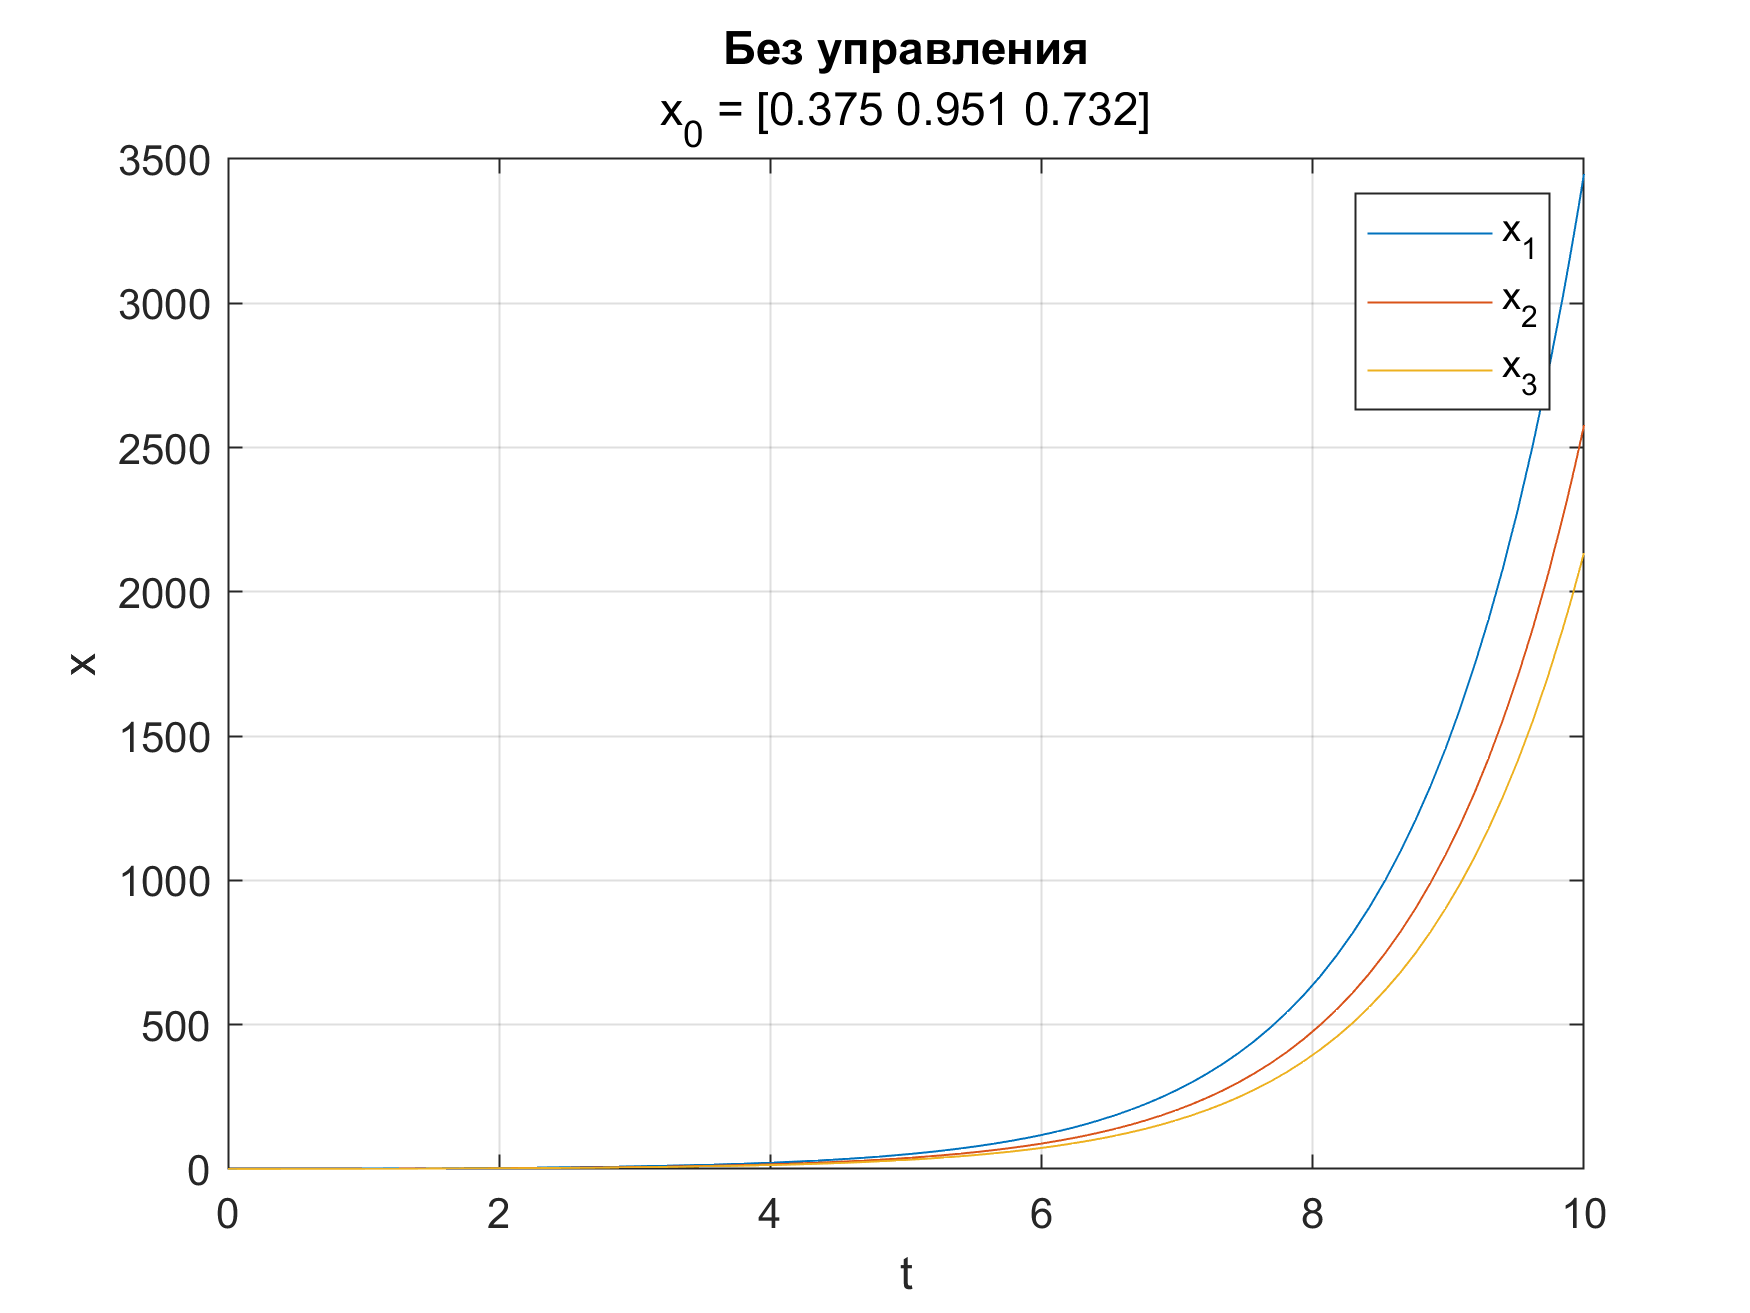
\includegraphics[width=0.7\textwidth]{no_control.png}
    \end{figure}
    Собственные числа матрицы $A$,
    \begin{equation*}
        \begin{aligned}
            \lambda_1 &= 0.84 \\
            \lambda_2 &= -7.67\\
            \lambda_3 &= -4.17
        \end{aligned}
    \end{equation*}

    Система очевидно неустойчива.

    \subsubsection*{С управлением. Асимптотическая устойчивость}
    \begin{figure}[H]
        \centering
        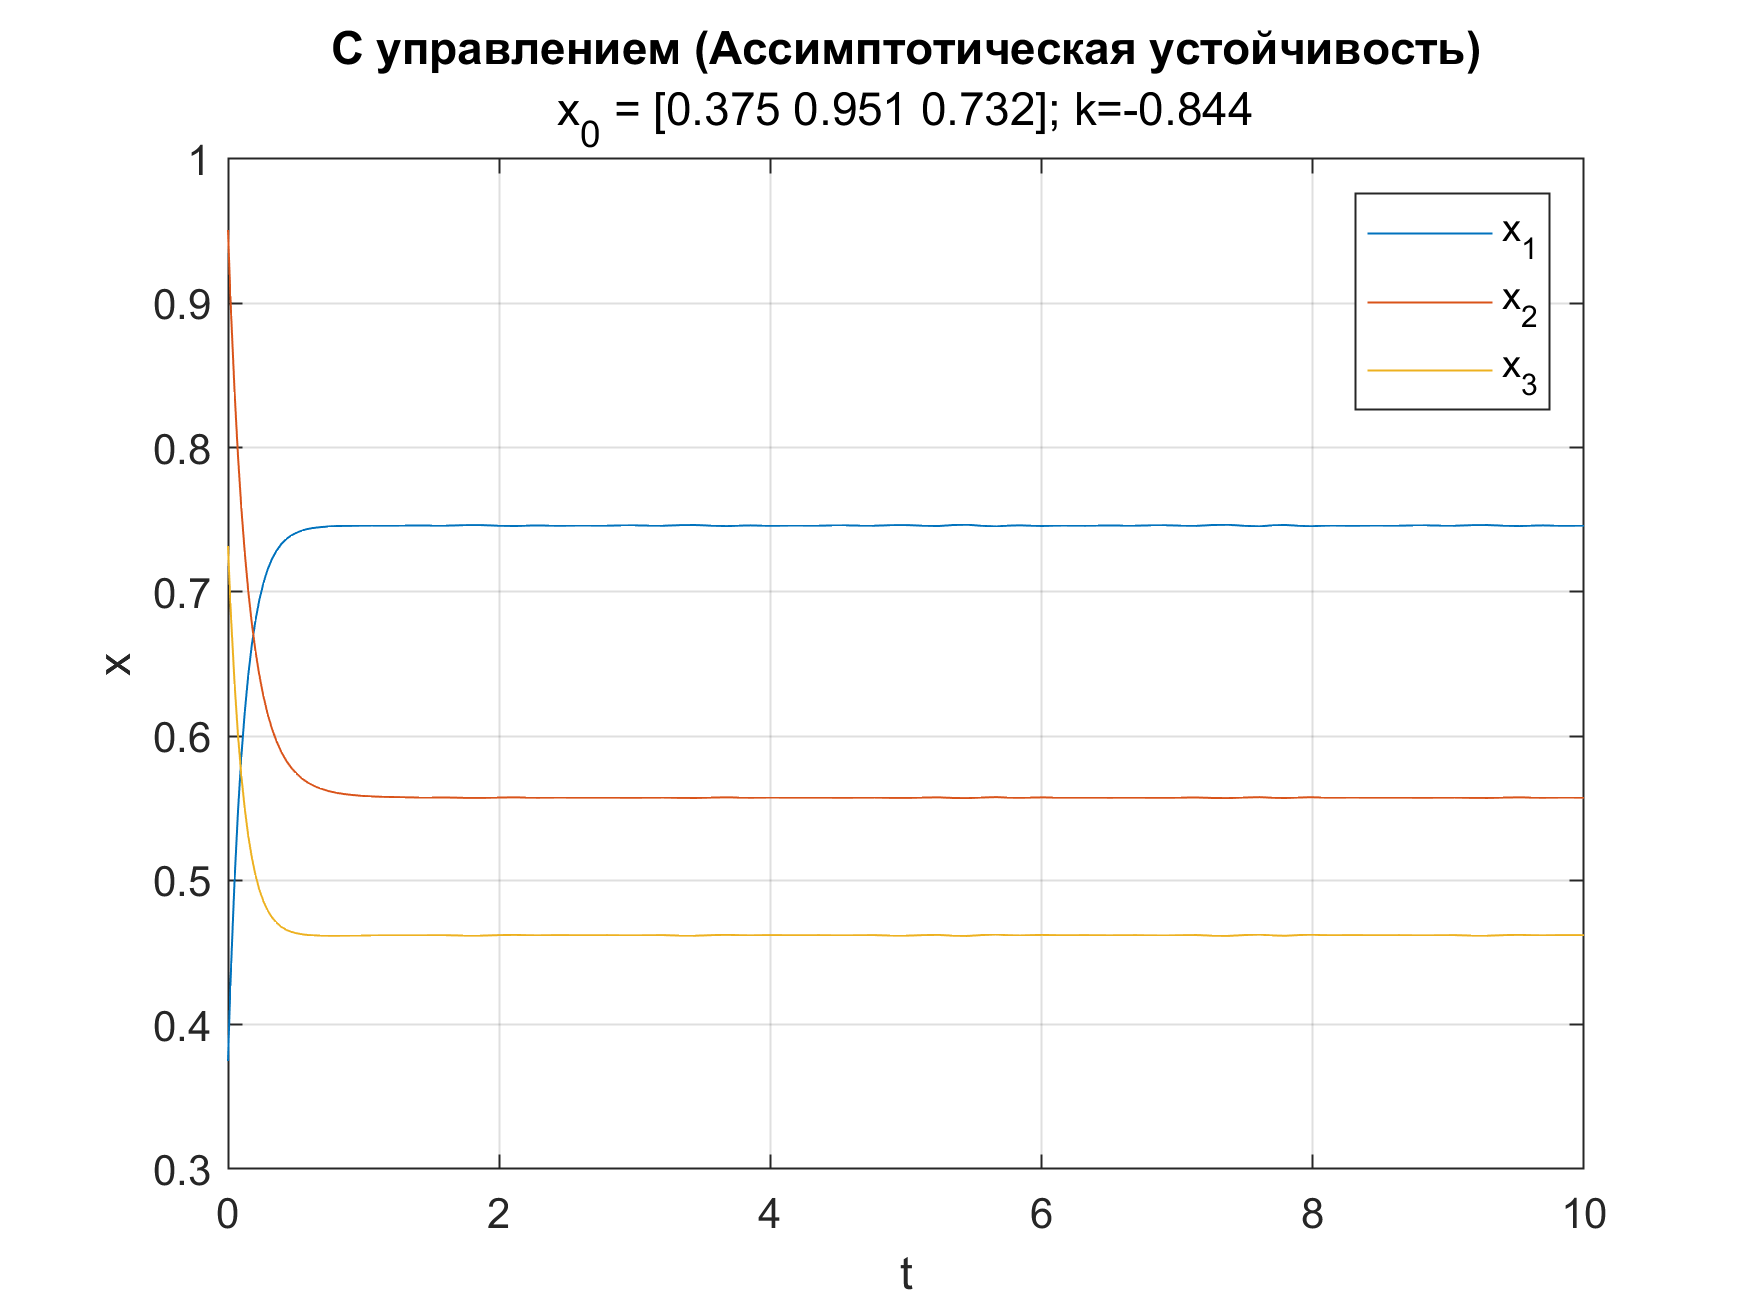
\includegraphics[width=0.7\textwidth]{assymp_control.png}
    \end{figure}
    Коэффициент усиления $k^* = -0.844$,\\
    Матрица замкнутой системы
    \begin{equation*}
        A^* = A + Bk^* =
        \begin{bmatrix}
            -3.844& 1& 5\\
            3& -4.844& 1\\
            3& 0& -4.844
        \end{bmatrix}
    \end{equation*}
    Собственные числа матрицы $A^*$,
    \begin{equation*}
        \begin{aligned}
            \lambda_1 &= 0 \\
            \lambda_2 &= -8.52\\
            \lambda_3 &= -5.01
        \end{aligned}
    \end{equation*}
    Ниже приведён код, использованный для выполнения задания.
    \inputminted[linenos, frame=single, breakanywhere]{octave}{../src/L1T3.m}
\end{document}
